\documentclass[10pt,twocolumn,letterpaper]{article}

\usepackage{cvpr}
\usepackage{times}
\usepackage{epsfig}
\usepackage{graphicx}
\usepackage{amsmath}
\usepackage{amssymb}
\usepackage{subcaption}

% Include other packages here, before hyperref.

% If you comment hyperref and then uncomment it, you should delete
% egpaper.aux before re-running latex.  (Or just hit 'q' on the first latex
% run, let it finish, and you should be clear).
\usepackage[pagebackref=false,breaklinks=true,letterpaper=true,bookmarks=false]{hyperref}

\cvprfinalcopy % *** Uncomment this line for the final submission

\def\cvprPaperID{****} % *** Enter the CVPR Paper ID here
\def\httilde{\mbox{\tt\raisebox{-.5ex}{\symbol{126}}}}

% Pages are numbered in submission mode, and unnumbered in camera-ready
\ifcvprfinal\pagestyle{empty}\fi
\begin{document}

%%%%%%%%% TITLE
\title{Cdiscount Final Project Report}

\author{Steven Jorgensen\\
Michigan State University \\
{\tt\small jorgen72@mu.edu}
% For a paper whose authors are all at the same institution,
% omit the following lines up until the closing ``}''.
% Additional authors and addresses can be added with ``\and'',
% just like the second author.
% To save space, use either the email address or home page, not both
\and
Matthew Andres Moreno\\
Michigan State University\\
{\tt\small mmore500@msu.edu}
\and
Ian Whalen\\
Michigan State University \\
{\tt\small whalenia@msu.edu}
}


\maketitle
%\thispagestyle{empty}

%%%%%%%%% ABSTRACT
\begin{abstract}
Online European retailer Cdiscount maintains an online catalog of 30 million products.
Cdiscount could achieve greater efficiency in managing its catalog of products by automating the product classificiation process. 
Cdiscount organizes its products into more than 5,000 categories, posing an extreme multi-category classification scheme problem.
We aim to develop an approach that leverages data made available by the retailer to allow for accurate, automated cataloging of products based on their images.
We use existing convolutional neural network techniques (CNN) to classify images and investigate how to best exploit the hierarchical nature of the Cdiscount categorization scheme to reduce the complexity of the problem.
Specifically, we use a subset of the cDiscount dataset to compare the performance of an approach employing a hierarchically nested set of models to the performance of an approach using a single model. 
We find that our method of exploiting the hierarchical nature of the data performs worse than the traditional single model approach on a smaller-scale multi-category product classification problem, most likely due to overfitting to training data.
\end{abstract}


%%%%%%%%% BODY TEXT
\section{Background}

\subsection{Problem Description}
\begin{figure}
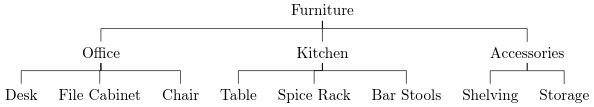
\includegraphics[width=\columnwidth]{img/hierarchy}
\caption{
Illustration of cDiscount's hierarchical classification scheme.
}
\label{fig:hierarchy}
\end{figure}

Cdiscount is one of France's largest e-commerce companies, selling everything from trampolines to televisions.
As the company grows, so does the number of different products they offer for sale.
In the past 2 years alone, they have added over 20 million new products to their catalog \cite{cDiscountKaggle}. 
The company uses a three-tier hierarchical classification system to organize its wares.
All products are assigned to a single high-level category.
This high-level categorization, such as such as ``furniture'' or ``electronics,'' is analogous to what department the product might be found in a traditional brick-and-mortar retailer. 
Within each department, products are organized into mid-level categories.
Within the high-level furniture categorization, for example, products are assigned to office, kitchen, accessories, etc. categories.
Finally, within each mid-level category, products are assigned to a single low-level category.
In the furniture department, for example, within the mid-level office categorization products are considered either a desk, a file cabinet, a chair, etc.
The categorization scheme is strictly hierarchical.
Each product belongs to a single low, mid, and high-level category; 
All products belonging to the same low-level category belong to the same mid-level category and all products belonging to the same mid-level category belong to the same high-level category.
Figure \ref{fig:hierarchy} overviews Cdiscount's product classification scheme.

Given the scale of Cdiscount's offerings, ensuring that each and every product is classified correctly is a challenging task.
Currently, Cdiscount uses machine learning text classification methods to categorize their wares.
To improve the accuracy of their classification methods, they would like to begin using images, rather than text, to categorize products.
To this end, Cdiscount sponsored a competition on the data science platform Kaggle to develop methods that automatically categorize products based on their images.
As part of this competition, they made available a data set with over 15 million images ranging over 5,000 categories.

\subsection{Data Set}

\begin{figure}
    \centering
    \begin{subfigure}[t]{0.33\columnwidth}
        \centering
        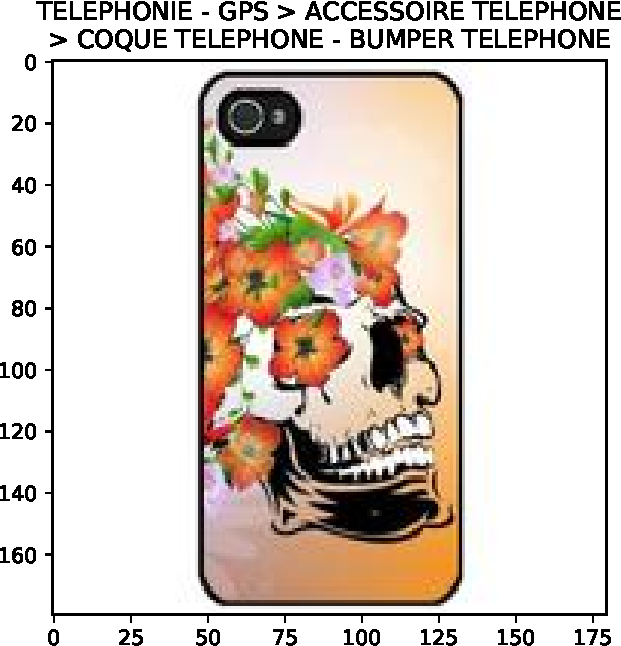
\includegraphics[width=\textwidth]{img/img-0-0}
        \caption{}
    \end{subfigure}%
    ~ 
    \begin{subfigure}[t]{0.33\columnwidth}
        \centering
        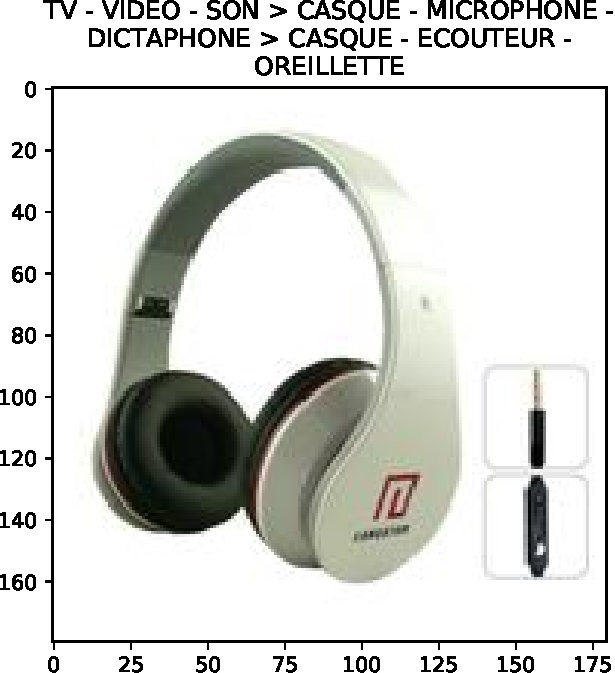
\includegraphics[width=\textwidth]{img/img-12-0}
        \caption{}
    \end{subfigure}%
    ~ 
    \begin{subfigure}[t]{0.33\columnwidth}
        \centering
        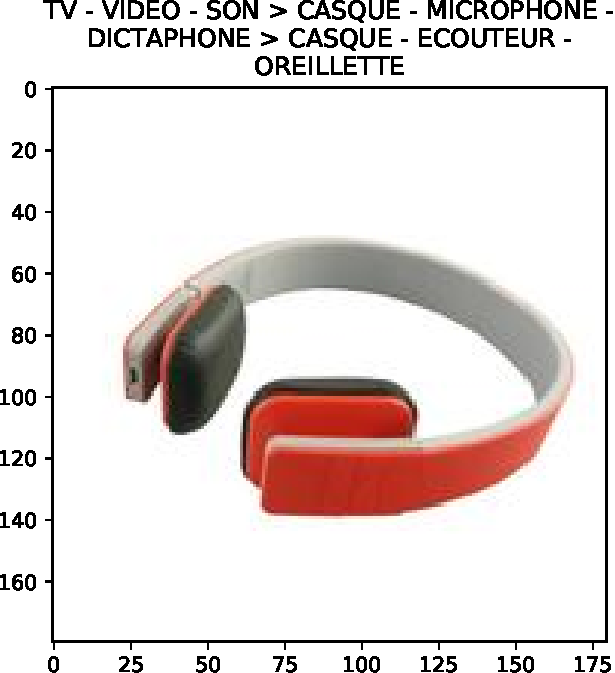
\includegraphics[width=\textwidth]{img/img-12-1}
        \caption{}
    \end{subfigure}
	\caption{
Images (a), (b), and (c) are three example training examples.
Image (a) is from a top level category different from images (b) and (c) (and therefore from different second and third categories, as well).
Images (b) and (c) are of the same product, and therefore from the same first, second, and third level categories.
Only some products, not all, have more than one associated image.
}
	\label{fig:example-images}
\end{figure}
\begin{figure}

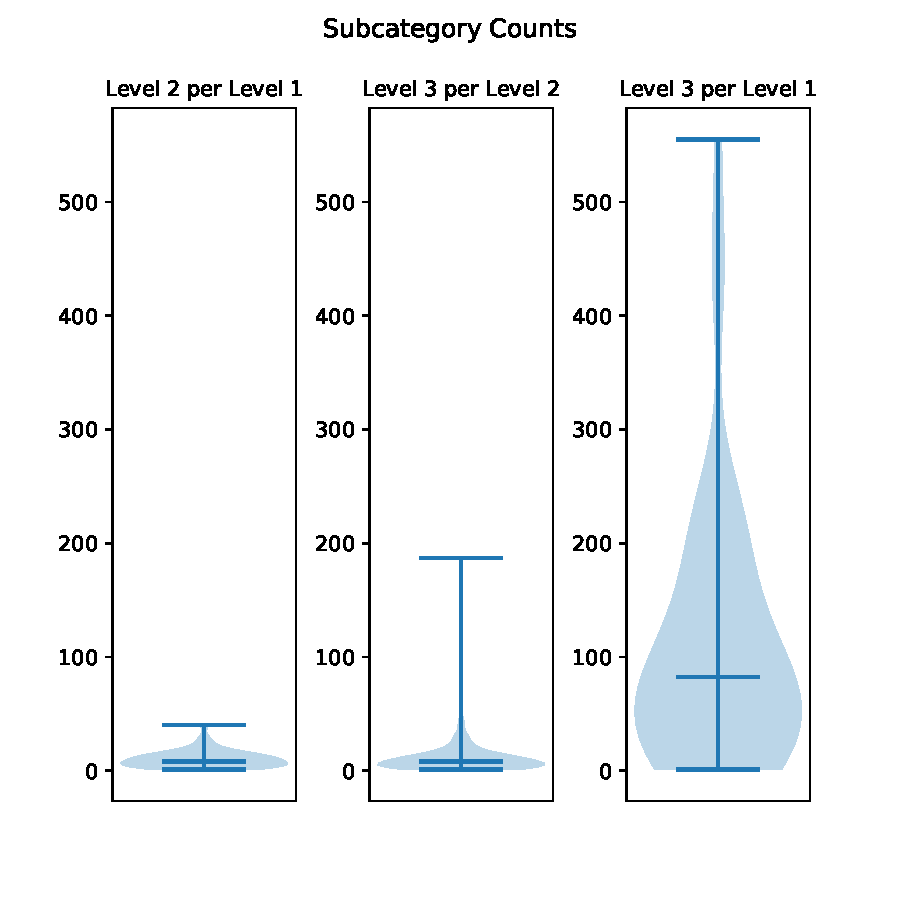
\includegraphics[width=\columnwidth]{img/catcount}
\caption{
This violin plot compares hierarchical category branching in the Cdiscount dataset.
The leftmost subplot presents the distribution of the number of second level subcategories in each top-level category.
The middle subplot presents the distribution of the number of third (bottom) level subcategories in each second level category.
The rightmost subplot presents the distribution of the number of bottom level subcategories in each first level category.
Going from first to second level and second to third level, categories branch by a median factor of approximately 10. 
From first to third level, categories branch by a median factor of approximately 100.
All three branching factor distributions have long right tails.
For example, going from second to third level, some categories are observed to branch by a factor of more than 150.
In all three subplots, horizontal bars mark the 0, 50, and 100th percentile counts.
}
\label{fig:catcount}

\end{figure}
\begin{figure}
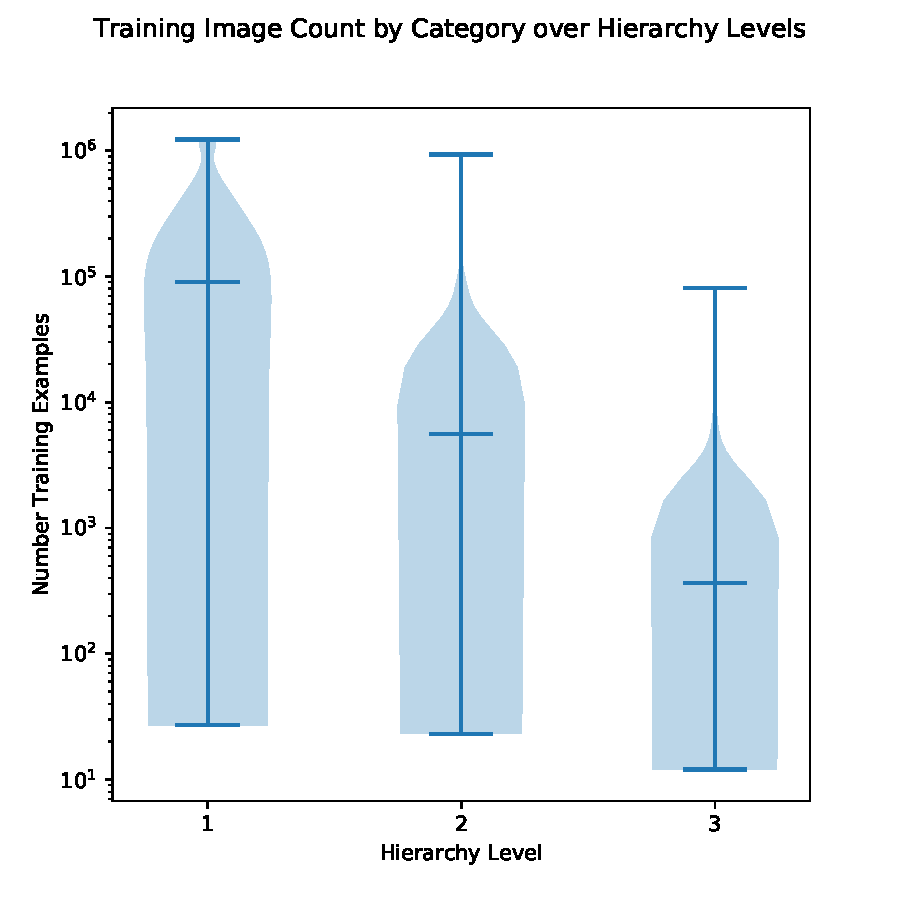
\includegraphics[width=\columnwidth]{img/datacount}
\caption{
This violin plot compares the number of training examples available for first (top) level categorizations, second level categorizations, and third (bottom) level categorizations.
As would be expected, the median training data count is highest for first level categories and lowest for third level categories.
On all three hierarchical levels, training data is distributed unevenly between categories.
For example, although the median top level category has approximately $10^5$ training examples, some have fewer than 100.
In all three subplots, horizontal bars mark the 0, 50, and 100th percentile counts.
}
\label{fig:datacount}
\end{figure}

Cdiscount has made an extensive dataset available through the data science platform Kaggle.
This dataset includes the full hierarchical categorization scheme used by Cdiscount and a listing of over 9 million products.
Each product has a unique ID, the ID of the category it falls in, and one to four images of that product.
The dataset comes divided into training and testing datasets, with the training set describing approximately 7 million products and the testing set describing approximately 2 million products.
Figure \ref{fig:example-images} shows example images from the Cdiscount dataset.
In this dataset, each image has 3 different levels of categorization, making this a challenging multi-classification problem.

Figure \ref{fig:catcount} shows the distribution of category-to-subcategory branching.
Figure \ref{fig:datacount} shows the distribution of availability of training data over all categories in each hierarchy level.
As described in the figure captions, the categorical branching factors and data availabilities vary widely across the dataset.
These irregularities make the Cdiscount challenge more difficult: some categories have many fewer training examples than other categories at the same hierarchy level and some categories have many more subcategories than others.



\section{Methods}
\begin{figure}
\centering
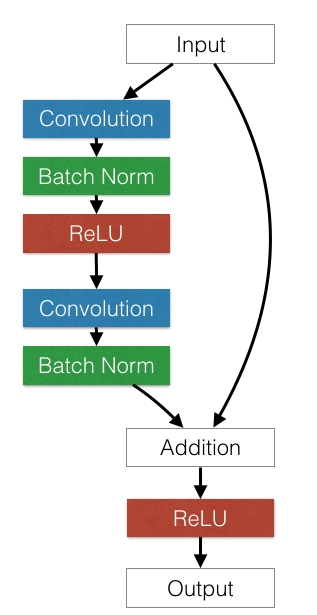
\includegraphics[width=0.4\columnwidth]{img/resnet}
\caption{
ResNet networks are characterized by skip connections, each of which bypasses several convolution layers \cite{gross2016training}.}
\label{fig:resnet}
\end{figure}

Our approach utilizes transfer learning, a well documented technique in the Deep Learning community as well as the broader field of Artificial Intelligence \cite{pan2010survey}.
Transfer learning involves repurposing models built for related, but distinct, problems. The original models serve as starting points for new models to be trained from.
This allows us to exploit knowledge gained from the original problem, without having to go through the process of learning it again in the new model. 
To incorporate transfer learning into our project, we utilize the ResNet \cite{he2016deep} architecture as a static feature extractor and train a single final fully connected layer to perform classification.
In some experiments, we perform fine tuning over all of the ResNet component's parameters in addition to the single final fully connected layer.
The ResNet architecture is designed for image classification and detection problems.
Deep feed-forward convolutional networks can suffer from a vanishing gradient problem where training stagnates due to error signal dissipation \cite{gross2016training}.
The ResNet architecture addresses this problem by including skip connections, each of which bypasses several convolutional layers \cite{he2016deep}.
At the end of a residual block, the output of the convolutional layers and the skip connection are summed \cite{gross2016training}.
By providing a direct shortcut for error signal to backpropagate through the network, these skip connections help to address the vanishing gradient problem.
Figure \ref{fig:resnet} provides a schematic depiction of a residual block.
ResNet architectures are composed of many such blocks.

\subsection{Preprocessing}

To meet the assumptions of the pretrained model components we used, we scaled images to 224 pixels by 224 pixels and performed the following channel normalizations, where $r$, $g$, and $b$, correspond to the red, green, and blue channels respectively:
\begin{align*}
r
&\sim
\mathcal{N}(0.485, 0.229) \\
g
&\sim 
\mathcal{N}(0.456, 0.224) \\
b
&\sim
\mathcal{N}(0.406, 0.225).
\end{align*}

To keep our work computationally tractable we work with just a subset of the entire Cdiscount dataset.
We restrict our work to two high-level categories and 20 of each high-level category's low-level categories.
We arbitrarily chose furniture and electronics as our high-level categories and then chose low-level categories to include based on the availability of adequate training data.
This reduced dataset comprises approximately 20,000 images, which were distributed roughly evenly between low-level categories.
Each low-level category had between 300 and 500 training examples.


\subsection{Approaches}
\begin{figure}
    \centering
    \begin{subfigure}[t]{0.55\columnwidth}
        \centering
        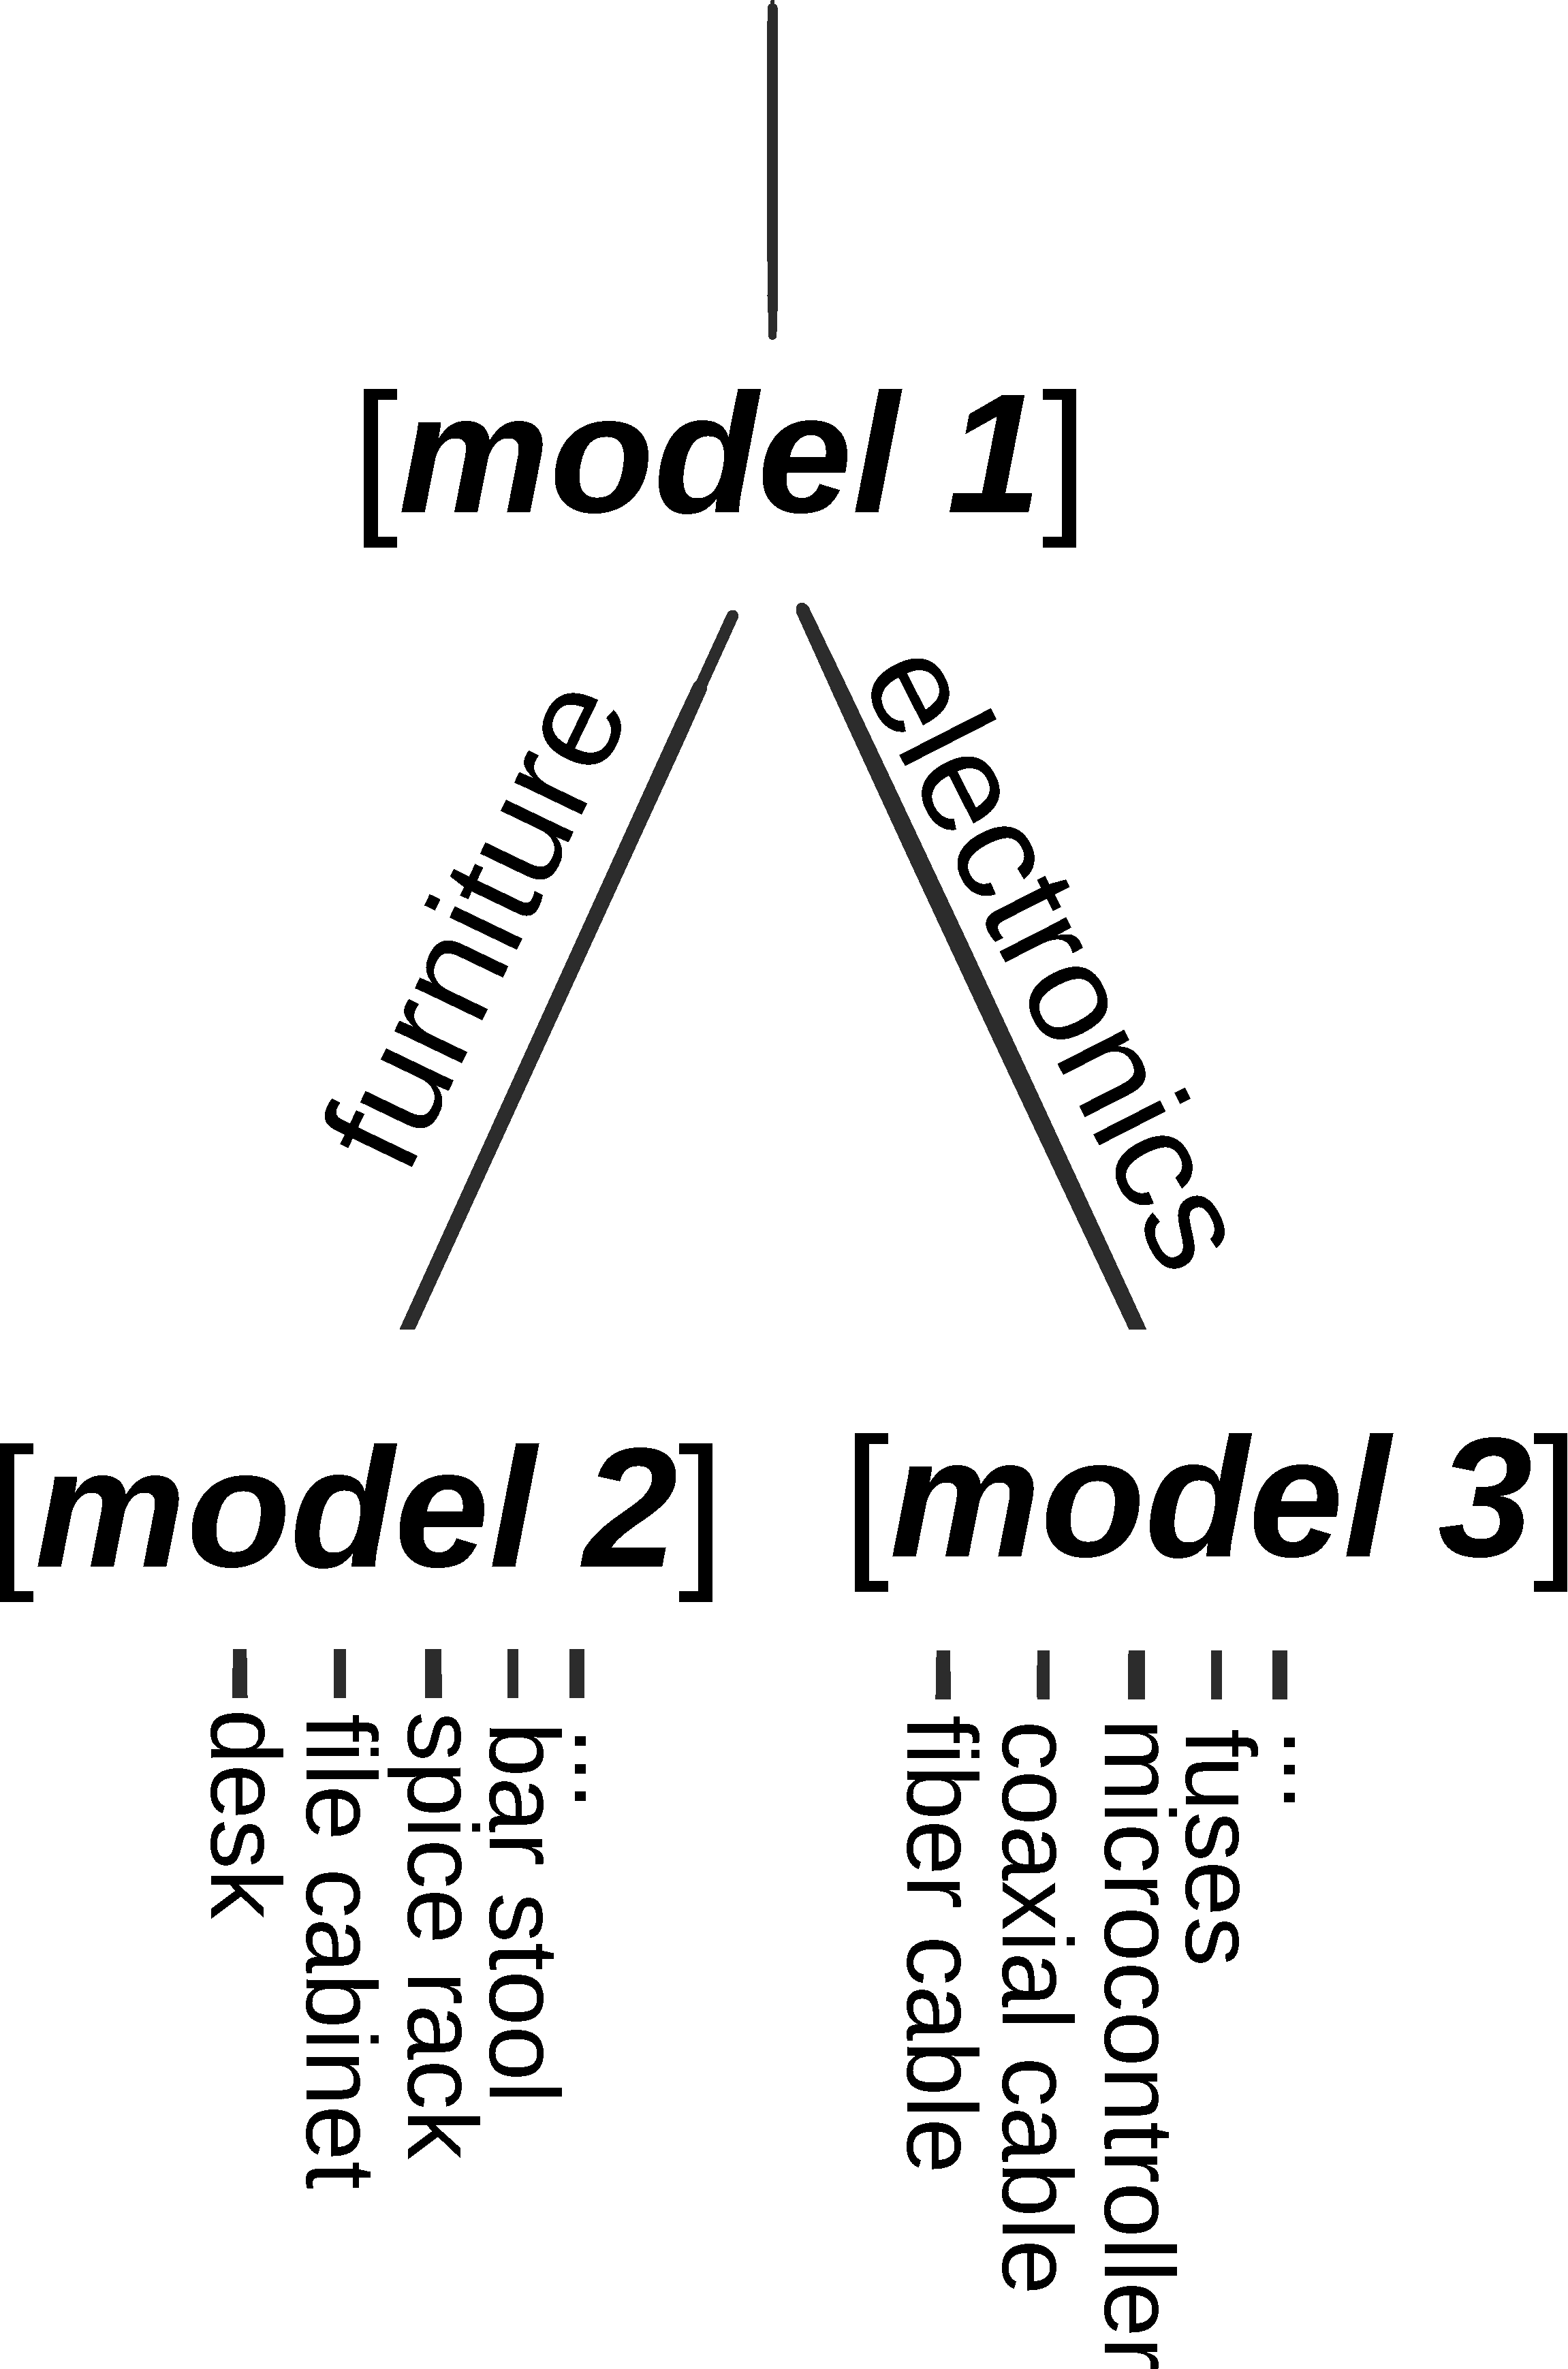
\includegraphics[width=\textwidth]{img/nested}
        \caption{nested models}
    \end{subfigure}%
    ~~~~~
    \begin{subfigure}[t]{0.40\columnwidth}
        \centering
        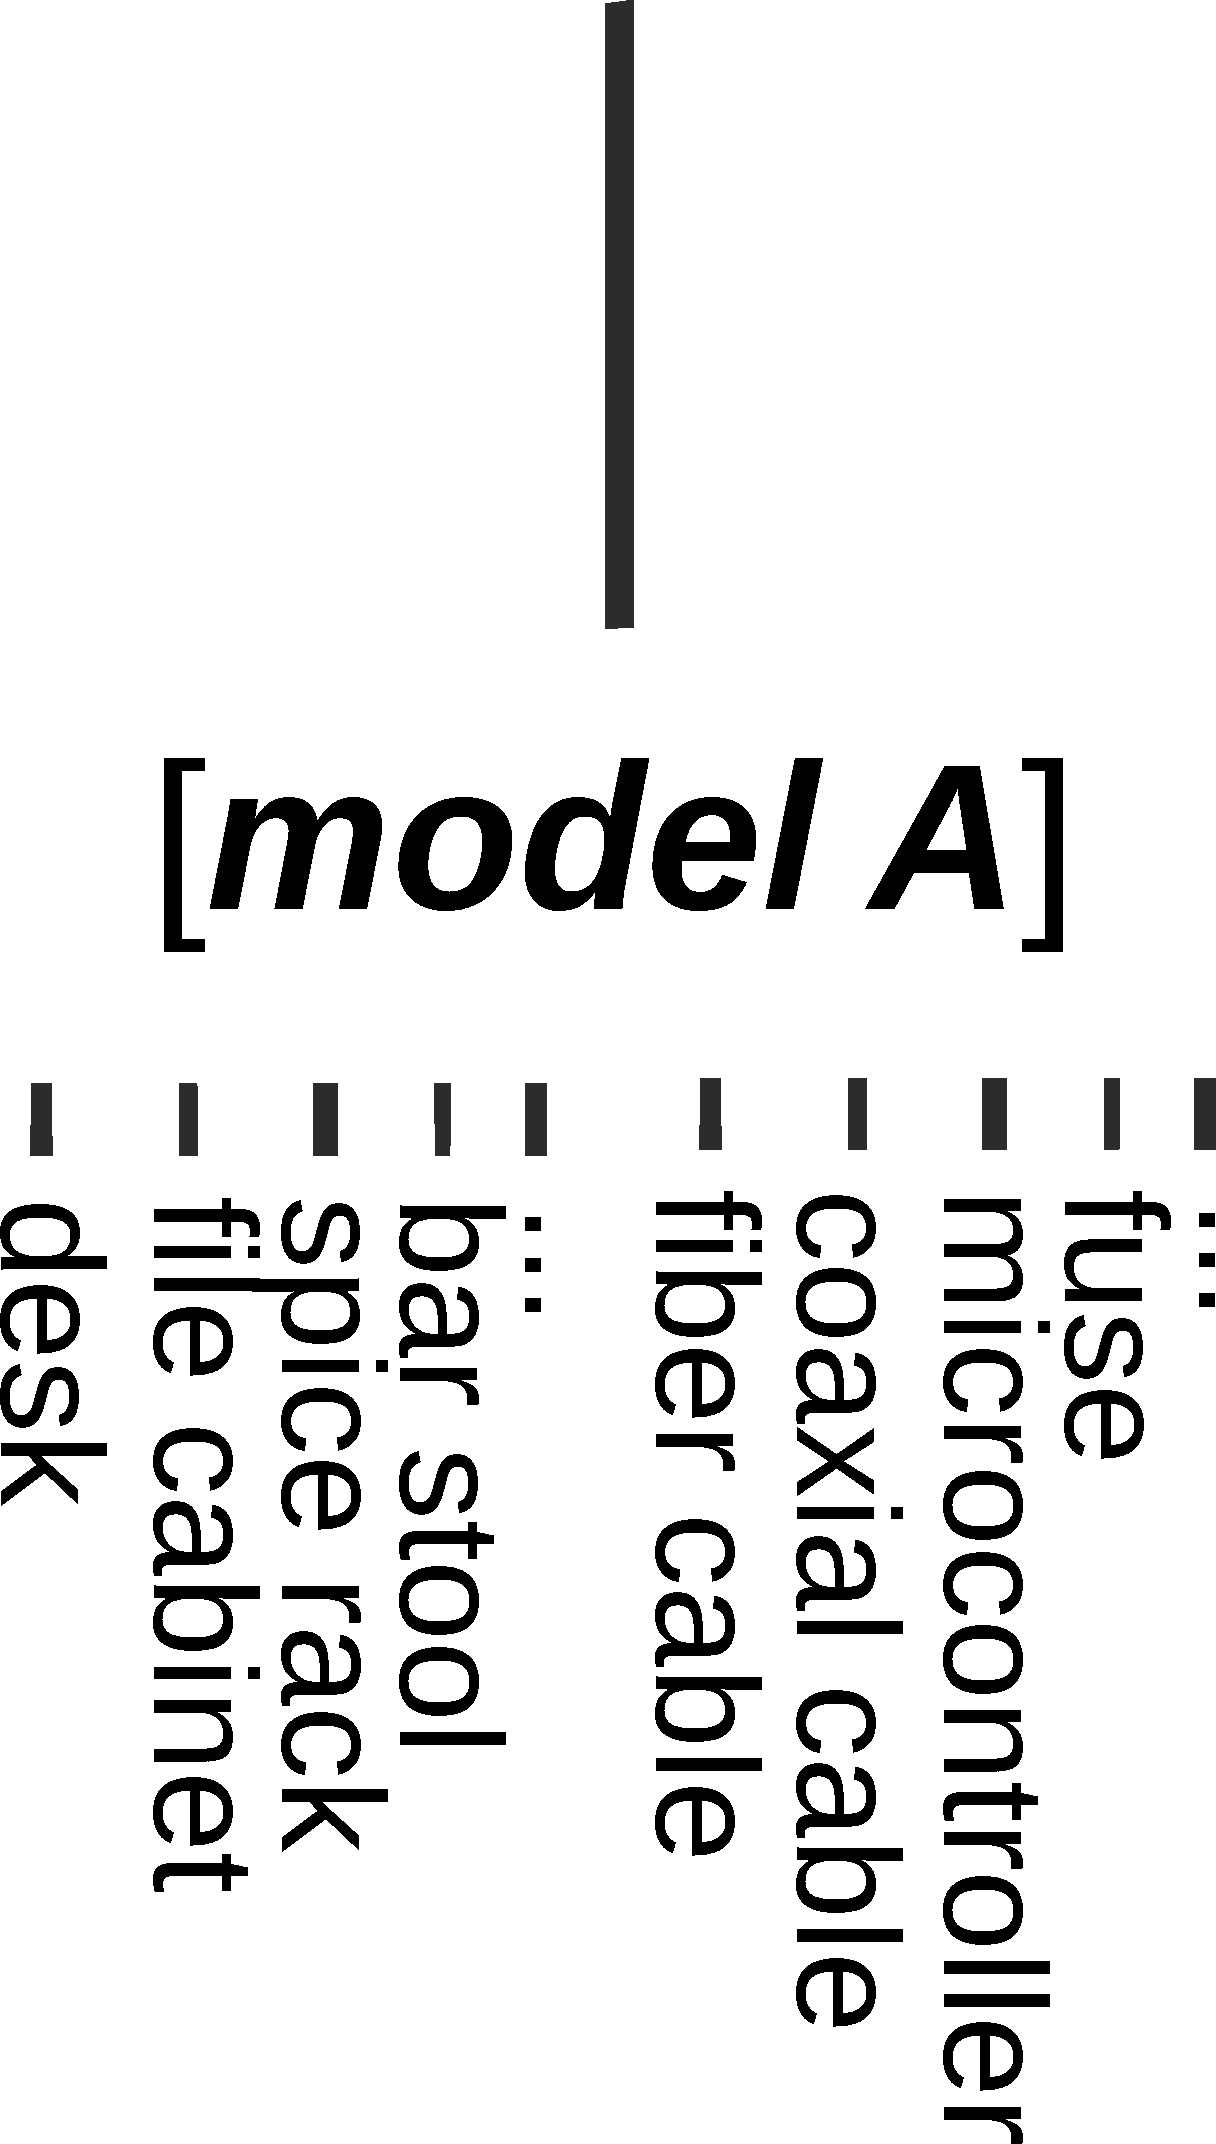
\includegraphics[width=\textwidth]{img/flat}
        \caption{flat model}
    \end{subfigure}
	\caption{
Schematic diagrams of the two approaches compared in this paper.
}
	\label{fig:approaches}
\end{figure}

We set out to compare the performance of two approaches to hierarchical image classification.
The first approach uses an ensemble of three models --- 1, 2, and 3 --- to perform classification.
Model 1 performs a classification between high-level categories.
With our reduced dataset, this is a binary classification.
We call this model the binary classification model.
Model 2 performs a classification between low-level categories for images classified by model 1 as belonging to a particular high-level category, in our case furniture.
We call this model the furniture-only model.
Model 3 performs a classification between low-level categories for images classified by model 1 as belonging to the other high-level category, in our case electronics.
We call this model the electronics-only model.
With our reduced dataset, models 2 and 3 both perform 20-class classification.
We refer to this approach the hierarchical models approach.

The second approach uses a single model to directly classify images between all low-level categories.
With our reduced dataset, this model performs 40-class classification.
Given the strictly hierarchical nature of cDiscount's classification scheme, the higher-level classifications of the image can be directly inferred from the low-level classification performed under this second approach. 
We call this approach the flat model approach.
Figure \ref{fig:approaches} provides a side-by-side schematic comparison of the hierarchical models and the flat model approaches.

\subsection{Implementation}

We use PyTorch and Torchvision to implement our experiments \cite{paszke2017pytorch}.
We used the ResNet18 model available through Torchvision, which has 11,689,512 trainable parameters when we perform fine tuning.
The final classification layer has 20,480 parameters for the flat model, 1,024 parameters for the binary classification model, and 10,240 parameters for the furniture-only and electronics-only models.  
The flat approach employs just one ResNet18 model.
However, the hierarchical approach employs three ResNet18 models and therefore entails three times the number of trainable parameters. 
We trained our models on a Google Cloud Compute virtual machine with a Nvidia Tesla K80 GPU.
Training our models consumed a total of 24 hours of compute time with this setup.

The scripts we used to analyze and visualize the Cdiscount dataset are hosted at \url{https://github.com/mmore500/cdiscount-datavis}.
Our code for dataset preparation, model design, model training, and comparison of classification accuracy between the flat model and the hierarchical models approaches is hosted at \url{https://github.com/ianwhale/cse891}.


\section{Results}
% * <mmore500.login@gmail.com> 2017-12-13T20:06:31.427Z:
%
% ^.

\begin{figure}
    \centering
    \begin{subfigure}[t]{0.5\columnwidth}
        \centering
        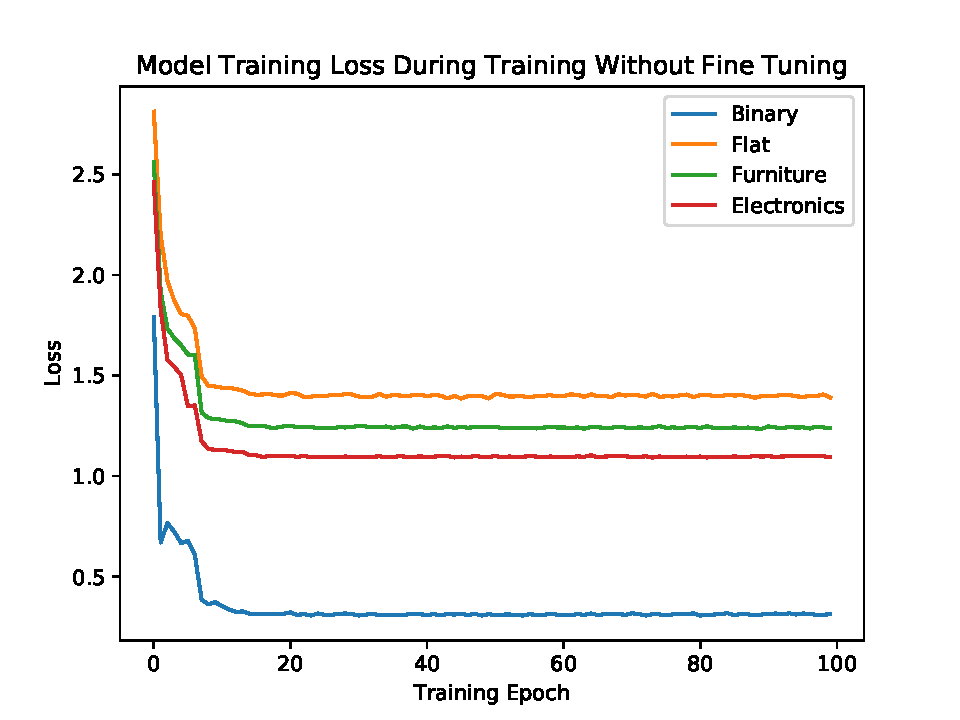
\includegraphics[width=\textwidth]{img/false_losses_train}
        \caption{}
    \end{subfigure}%
    ~ 
    \begin{subfigure}[t]{0.5\columnwidth}
        \centering
        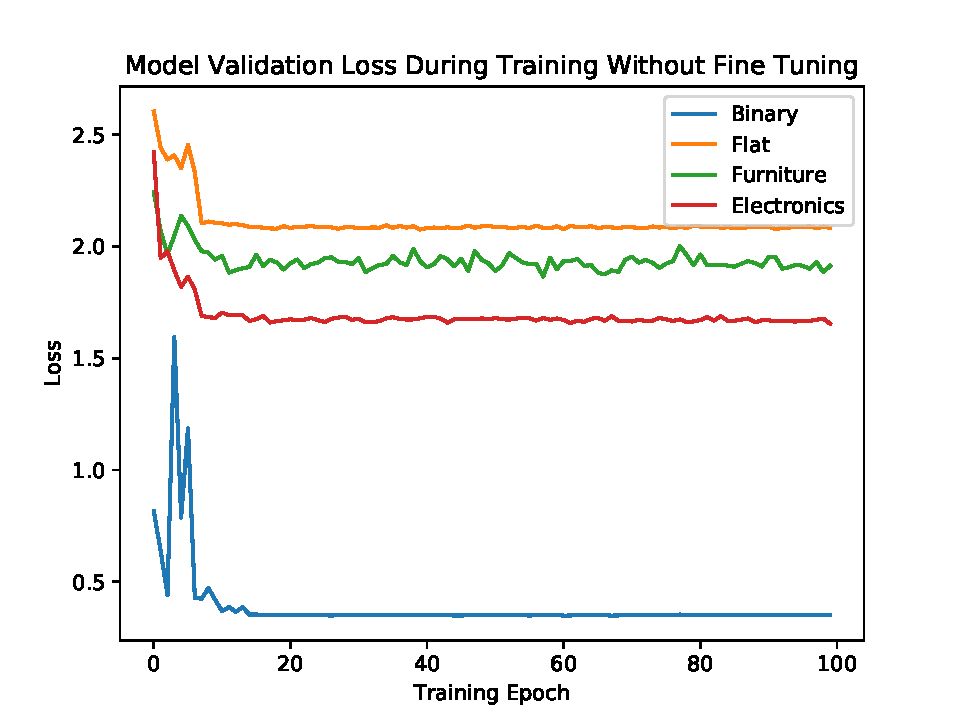
\includegraphics[width=\textwidth]{img/false_losses_val}
        \caption{}
    \end{subfigure}%
	\caption{
Loss values of our models during training without fine tuning.
Subfigure (a) displays training loss by epoch.
Subfigure (b) displays testing loss by epoch. 
}
	\label{fig:false_losses}
\end{figure}
\begin{figure}
    \centering
    \begin{subfigure}[t]{0.5\columnwidth}
        \centering
        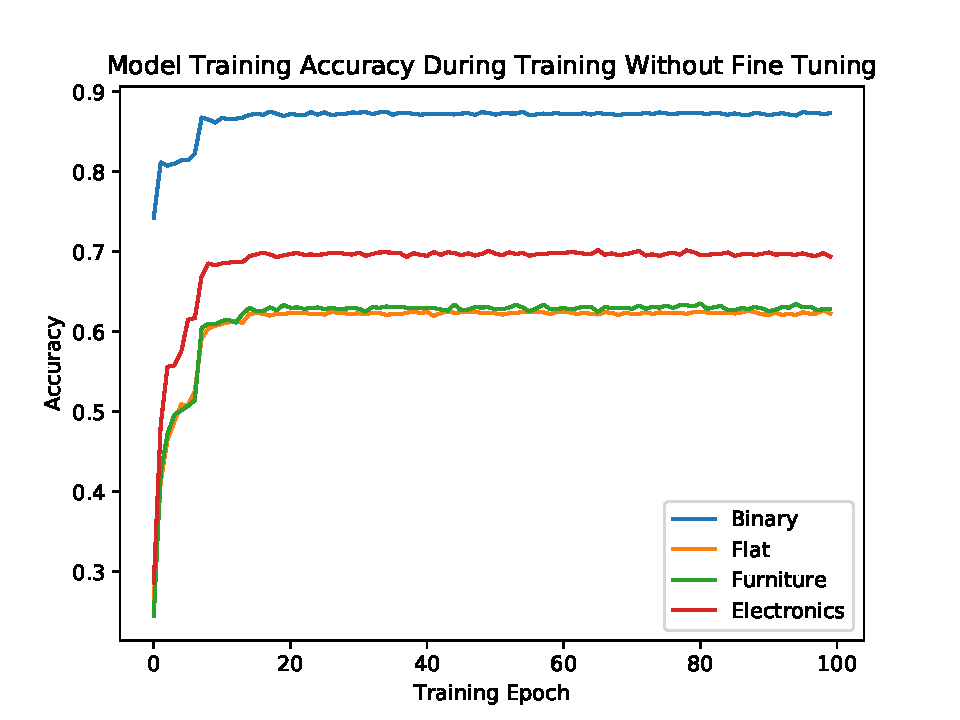
\includegraphics[width=\textwidth]{img/false_accs_train}
        \caption{}
    \end{subfigure}%
    ~ 
    \begin{subfigure}[t]{0.5\columnwidth}
        \centering
        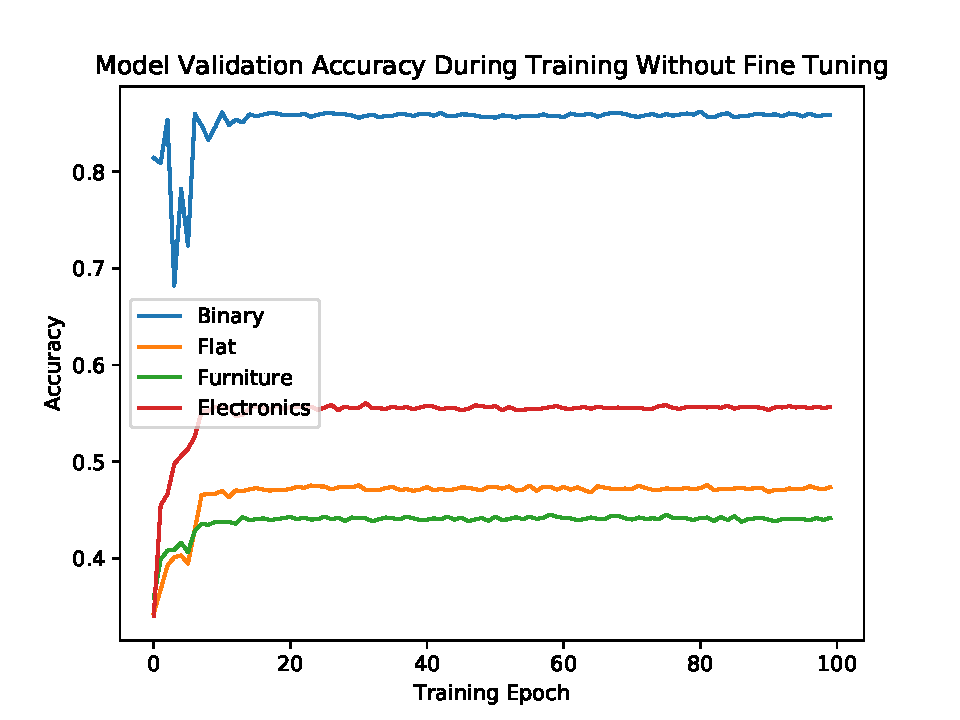
\includegraphics[width=\textwidth]{img/false_accs_val}
        \caption{}
    \end{subfigure}%
	\caption{
Classification accuracy of our models during training without fine tuning.
Subfigure (a) displays training accuracy by epoch.
Subfigure (b) displays testing accuracy by epoch. 
}
	\label{fig:false_accs}
\end{figure}
\begin{figure}
    \centering
    \begin{subfigure}[t]{0.5\columnwidth}
        \centering
        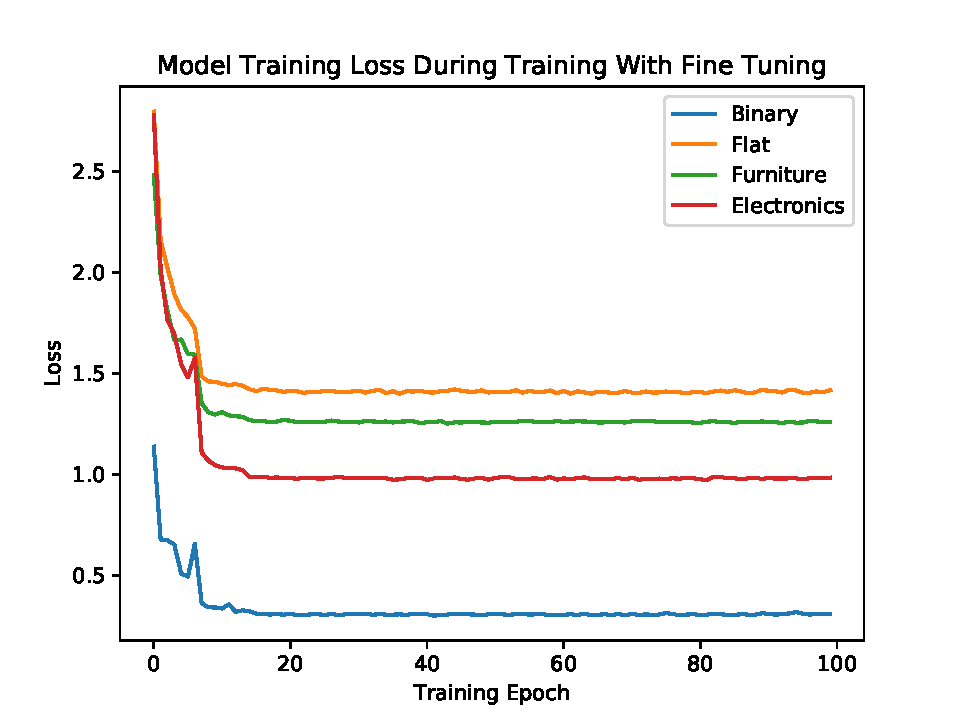
\includegraphics[width=\textwidth]{img/true_losses_train}
        \caption{}
    \end{subfigure}%
    ~ 
    \begin{subfigure}[t]{0.5\columnwidth}
        \centering
        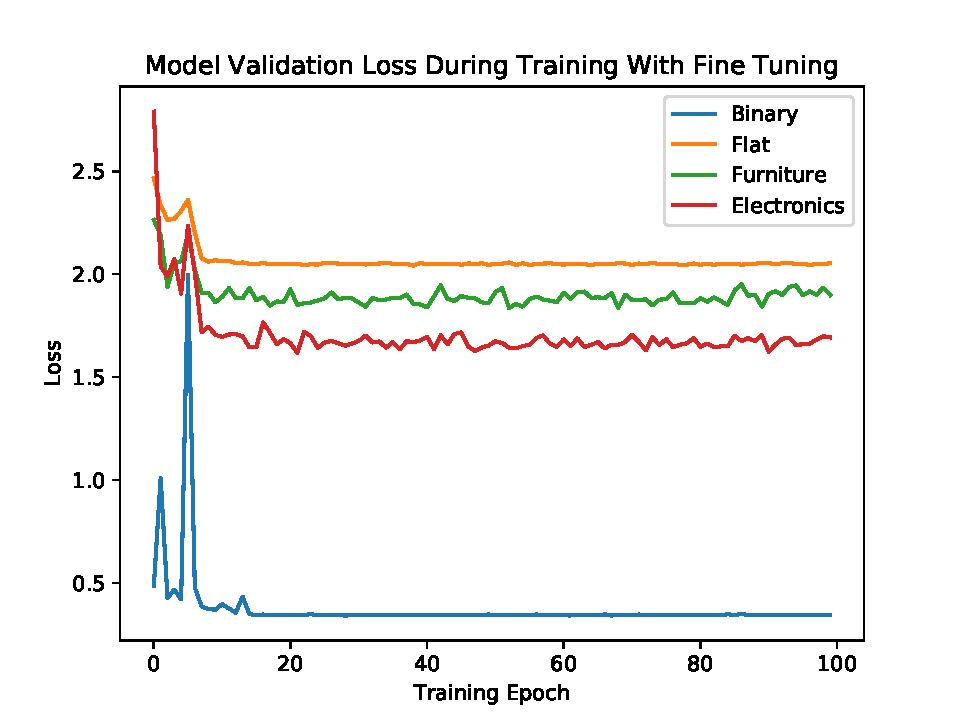
\includegraphics[width=\textwidth]{img/true_losses_val}
        \caption{}
    \end{subfigure}%
	\caption{
Loss values of our models during training with fine tuning.
Subfigure (a) displays training loss by epoch.
Subfigure (b) displays testing loss by epoch. 
}
\label{fig:true_losses}
\end{figure}
\begin{figure}
    \centering
    \begin{subfigure}[t]{0.5\columnwidth}
        \centering
        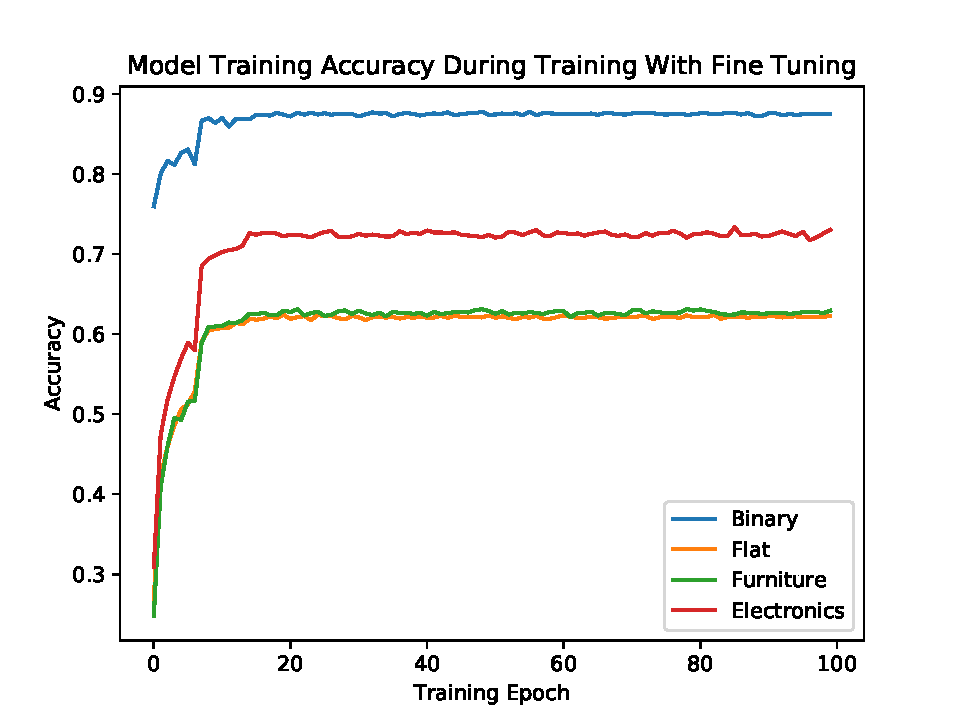
\includegraphics[width=\textwidth]{img/true_accs_train}
        \caption{}
    \end{subfigure}%
    ~ 
    \begin{subfigure}[t]{0.5\columnwidth}
        \centering
        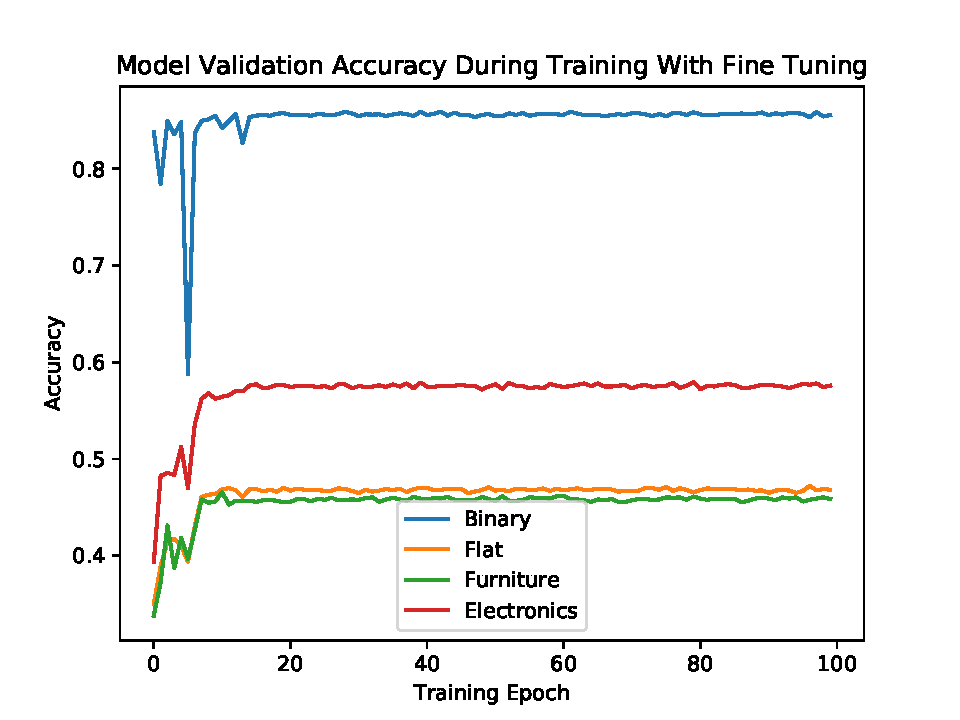
\includegraphics[width=\textwidth]{img/true_accs_val}
        \caption{}
    \end{subfigure}%
	\caption{
Classification accuracy of our models during training with fine tuning.
Subfigure (a) displays training accuracy by epoch.
Subfigure (b) displays testing accuracy by epoch. 
}
	\label{fig:true_accs}
\end{figure}
\begin{figure}
\begin{center}
\begin{tabular}{ c|c c } 
 ~ & Flat & Hierarchical \\
 \hline
 fine tuning & 0.5813 & 0.4076 \\ 
 no fine tuning & 0.5891 & 0.5540 \\ 
\end{tabular}
\end{center}
\caption{
Validation set classification accuracy of flat model and hierarchical models approaches with and without fine tuning.
}
\label{fig:acc_table}
\end{figure}

Figures \ref{fig:false_losses} and \ref{fig:true_losses} show training and testing loss by epoch for the four ResNet models that were trained (three for the hierarchical models approach, one for the flat model approach). 
Specifically, Figure \ref{fig:false_losses} documents loss by epoch for transfer learning without fine tuning and Figure \ref{fig:true_losses} documents loss by epoch for transfer learning with fine tuning.
In both cases, testing loss exceeds training loss to some extent for the flat, furniture, and electronics models, indicating that these models overfit the training data.
Based on the difference between training and testing loss, the extent of overfitting appears to be comparable both with and without fine tuning.
However, training and testing loss was very similar for the binary classification model both with and without fine tuning, suggesting this model did not as strongly overfit its training data.
Perhaps this reduced overfitting was due to a greater number of training examples being available per class because this model only catergorizes between two classes.

Figures \ref{fig:false_accs} and \ref{fig:true_accs} show training and testing classification accuracy by epoch for the four ResNet models that were trained.
Specifically, Figure \ref{fig:false_accs} shows classification accuracy by epoch for transfer learning without fine tuning and Figure \ref{fig:true_accs} shows classification accuracy by epoch for transfer learning with fine tuning.
In both cases, training accuracy significantly exceeds training accuracy for the flat, furniture, and electronics models, providing another indication that these models overfit the training data. 
As before, testing and training accuracies were more similar for the binary classification model with and without fine tuning, suggesting that this model did not as strongly overfit its training data.
Interestingly, the both with and without fine tuning testing classification accuracy for the electronics model significantly exceeded the testing classification accuracy for the furniture model, suggesting that discriminating between low-level furniture classes was a more difficult problem for our methods than discriminating between low-level electronics classes.
In fact, both with and without fine tuning classification accuracy for the furniture model was similar to that of the furniture model, even though the flat model must categorize between twice as many categories.
In some cases classification accuracy for the flat model seems to actually slightly exceed the classification accuracy for the furniture model.
The poor performance of the furniture-only classifier relative to the electronics-only classifier may be an artifact of the particular low-level furniture classes that we included in our reduced dataset or simply of the furniture low-level classes in general.
However, the sometimes slightly superior classification accuracy of the flat model is perplexing because the flat model must in fact perform the same furniture classifications as the furniture-only model.

Finally, Figure \ref{fig:acc_table} summarizes the classification accuracies of the flat model approach and the hierarchical models approach.
The flat model approach yielded better classification accuracy than the hierarchical models approach, both with and without fine tuning.
The hierarchical model performed somewhat comparably to the flat model without fine tuning but its classification accuracy suffered significantly when fine tuning was used while training its constituent models.

\section{Discussion}

As shown in Figure \ref{fig:acc_table}, the flat model approach outperforms the hierarchical models approach both with and without fine tuning.
We suspect that performance of the hierarchical models may be hindered by overfitting to training data.
The much poorer performance of the hierarchical models approach with the addition of fine tuning would support this hypothesis as fine tuning greatly increases the number of trainable parameters, providing a greater opportunity for overfitting to occur.
Although the binary classification component of the hierarchical models approach does not seem to suffer from significant overfitting, the furniture-only and electronics-only models certainly do.
The binary classification model was trained on roughly several thousand images per class.
The furniture-only and electronics-only models, however, were trained on just several hundred images per class, presenting a greater opportunity for overfitting.
Further, these furniture-only and electronics-only models had approximately the same number of example images per class as the flat model but twice as many trainable parameters per class compared to the flat model.
Thus, these components of the hierarchical models approach might be more prone to overfitting than the flat model. 
If overfitting in fact explains the poor performance of the hierarchical models approach, training techniques specifically designed to reduce overfitting could be used to improve the performance of the hierarchical models approach.
In particular, dropout and data augmentation like rotation, flipping, and the addition of random noise might prove helpful \cite{srivastava2014dropout, taylor2017improving}.
(The flat model approach, which also suffers from overfitting, would certainly stand to benefit from such interventions, too).

The poor performance of the hierarchical models approach might also be improved by addressing the poor performance of the furniture-only model relative to the electronics-only model hierarchical model.
A more systematic tuning of hyperparameter settings might improve the performance of the furniture-only model.
In particular, using a decaying learning rate or just a lower learning rate might improve model performance with fine tuning.
Trying other models for transfer learning such as VGG \cite{he2016deep} and inception net \cite{szegedy2015going} might also improve performance on the furniture-only classification task.   
Finally, these experiments should be repeated with other dataset reduction choices (i.e. with other high and low-level categories from the Cdiscount dataset) to ensure that furniture, electronics, and the particular low-level categories that were chosen were representative of the entire Cdiscount dataset.
Given the relatively poor performance of the furniture-only model, the performance of the hierarchical models approach might be better for other subsets of the Cdiscount dataset.  

The scale that we tested our two approaches at --- 40 low-level classes --- is not a particularly large multi-class classification problem \cite{deng2010does}.
The superior performance of the flat model approach compared to the hierarchical models approach we observed for this 40 class classification problem may not hold up on a larger multi-class classification problem, i.e. the entire Cdiscount 5000 class classification problem.
It would be interesting to compare the performance of these approaches on a larger multi-class classification problem.
However, even if the hierarchical models approach exhibits performance superior to the flat model at a larger scale, our results show that on smaller scale problems the flat model approach works best.
Thus, for hierarchical classification problems of intermediate scale, it would likely be necessary to try both approaches and select which to use based on testing performance.
Additionally, the hierarchical models approach, which required three separate classification models to be trained, is much more computationally expensive than the flat model approach.
Scaling the hierarchical models approach to the entire Cdiscount dataset, which includes 49 high-level categories, would require fifty models to be trained.
The much greater compute cost of the hierarchical models approach would need to be considered in any decision to use that approach in practice.

\section{Author Contributions}

All authors were collaboratively involved in the high-level design decisions made in this project.
However, for efficiency we divided labor implementing and documenting those high-level design decisions across different types of tasks that could be completed independently.


\noindent
\textit{Steven} Prepared data, ran statistical scripts on the data, spearheaded written reports, worked with Matthew to finalize model training for the four different types of models trained, and performed model training on Google Cloud Compute.

\noindent
\textit{Matthew} Created visualizations, compiled results, spearheaded written reports, wrote script to compare classification accuracies of flat model and nested models approaches, worked with Steven to finalize model training for the four different types of models trained.

\noindent
\textit{Ian} Subsetted and preprocessed data, created dataset iterator, spearheaded software installation logistics, prototyped model training, prepared and gave oral presentation. 




{\small
\bibliographystyle{ieee}
\bibliography{egbib}
}

\end{document}
